
    The research contributions of this thesis are based on a novel constraint
    programming approach on compiler intermediate representation.
    This chapter introduces the theoretical underpinnings of this approach,
    based on a mathematical model of static single assignment form (SSA).
    With the help of this model, concepts that are typically discussed on a
    programming language level are transferred onto the structurally simple,
    yet semtantically expressive class of SSA compiler intermediate
    representations.

    Constraint formulas on SSA respresentations initially appear to mimic
    pattern matching approaches on abstract syntax tree (AST) level.
    However, they quickly prove themselves to be vastly more expressive.
    Some consideration is necessary to handle search space explosion, but
    the reward are much more powerful recognition capabilities and the
    expression of higher level algorithmic structures, which are impossible to
    define syntactically on programming language level.
    Later chapters will explore the power of this approach in detail, by
    building a complete constraint programming language on top of the theory in
    this chapter, and by then using it to solve real compiler analysis problems.

    After defining a mathematical foundation of SSA form and introducing
    formalisms for the expression of basic contraint problems on top of it,
    several standard definitions from compiler theory are reformulated in the
    framework.
    This includes common graph properties, including the concept of domination,
    as well as control flow structures such as single entry single exit blocks.
    All of this lays the foundations for the succeeding chapter.

    Finally, for the practical application of constraint programming to compiler
    intermediate representation, efficient solver techniques are needed.
    The last section in this chapter discusses strategies for limiting
    compile time explosion and explores analogies of the described model to
    standard Satisfiability Modulo Theory (SMT) problems.
    This gives further insights into performance improvements and puts the
    work into a broader theoretical context.

\section{Introduction}

    Modern compilers for procedural languages such as
    C/C++, Fortran or JavaScript typically use a succession of different
    representations for the program during compilation.
    They can be grouped into categories and reflect the requirements of
    the compilation stages they are used in.
    \linebreak
    {\bf Front end representations} are close to the source program and
    naturally reflect the internals of the compiler front end, especially the
    parser.
    Typically, they are built on an abstract syntax tree representation with
    additional annotations, such as type information.
    In addition to encoding program logic, these representations are rich in
    information about syntactic and  stylistic choices of the programmer.
    They scale in complexity with the source language and further obscure the
    program semantics by not resolving complex language features, such as
    operator overloading.
    \linebreak
    {\bf Back end representations} are based on a model of the target hardware.
    These representations typically approach an assembly style format,
    exposing specific instruction set architectures of the hardware.
    Back end representations are concerned with problems that are removed from
    the algorithmic core of the user program, such as register allocation and
    instruction scheduling.
    \\
    {\bf Static Single Assignment} (SSA) form has emerged as a suitable
    representation in the middle end, which is traditionally responsible for
    applying complex optimising transformations.
    SSA abstracts away the complexities of both the source language and the
    target architecture, instead focusing on a relatively simple semantic
    description of the user program that enables reliable analysis and platform
    independent reasoning.
    It is these properties that also make it the natural representation for
    expressing algorithmic structures.

    Static Single Assignment is not a strictly defined or mathematically
    codified standard, but instead refers to a group of representations that
    share important characteristics,
    the eponymous SSA property being only one among them.
    Instruction sets, syntax and type systems of the different
    SSA intermediate representations vary considerably, depending on the
    requirements of the source languages (static or dynamic)
    and the operating constraints (just-in-time or ahead-of-time).
    Some prominent examples of compilers that utilize SSA for their
    optimisation passes include {\bf clang} (LLVM IR), {\bf gcc} (GIMPLE),
    {\bf v8 Crankshaft} (Hydrogen) and {\bf SpiderMonkey} (IonMonkey/MIR).
    Despite many differences, they share the same fundamental paradigms
    and many of the differences can be abstracted away as implementation
    specific details.

    Fundamentally, a program in single static assignment form is made up of
    functions, which are represented as sequences of instructions, grouped into
    basic blocks and operating on virtual registers.
    The control flow is handled via jump instructions at end of basic blocks.
    The virtual registers, within a function, can be assigned only at a single
    static location each, which has very useful implications as we will later
    see.
    As opposed to syntax-heavy representations, SSA form is a searialized
    program representation, where expressions have been turned into lists of
    instructions and control flow structures into lists of basic blocks.
    The following sections explore how this serial nature makes constraint
    programming concepts naturally applicable.

\subsection{Static Single Assignment Form}

\begin{figure}[t]
\centering
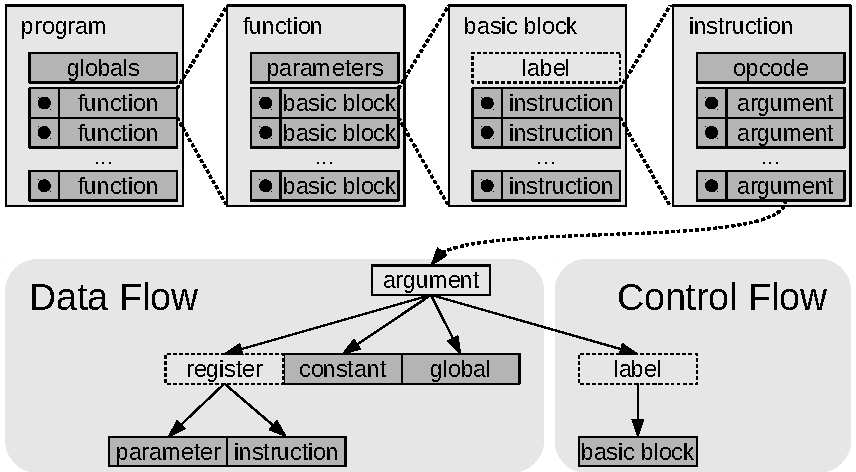
\includegraphics{figures/ssaoverview}
\caption{Structural overview of SSA: Programs are represented as hierarchies of
    lists. The SSA property makes registers implicit, values can be statically
    matched to defining instructions.}
\label{fig:ssaoverview}
\end{figure}

    SSA representations of programs are highly serialised, as shown in
    \autoref{fig:ssaoverview}:
    Programs are lists of functions, functions are lists of basic blocks,
    basic blocks are lists of instructions and instructions are most
    fundamentally lists of arguments.

    The individual instructions operate on an abstract machine, which provides
    an unlimited number of identical registers and a well defined instruction
    set.
    The control flow is expressed as branch instructions, which direct the
    execution conditionally or unconditionally to other basic blocks.
    Basic blocks may have labels or be identified simply by enumerating them.
    Instruction arguments can be registers, constants or globals and branch
    instructions additionally take basic block labels.
    Instructions can write their result into a single output register.
    Branch instructions always terminate a basic block, control flow divergence
    within basic blocks is not possible.

    The static single assignment property stipulates that within a function,
    no register can be written at more than a single static location.
    This makes the data dependencies between the instructions explicit, as it
    implies that registers can be identified directly with the instructions that
    write to them.
    The registers themselves can therefore be considered implicit, with only the
    data flow between instructions required to recover them.

    In the presence of dynamic control flow behaviour in the program, most
    simply in the case of a conditional branch, it is evidently not possible to
    match values to producing instructions statically.
    This is resolved with {\em phi} instructions.
    These instructions select a value from several arguments depending on the
    previously executed basic block, i.e.\ depending on the branch from where
    the execution reached the basic block containing the phi node.

\subsection{Example of Static Single Assignment Form}

    \autoref{ssaexample} shows many of the key features of static single
    assignment form and how they naturally emerge from simplification steps of
    the source code of procedural languages.
    This is demonstrated on an example function ``{\tt sqrt}'' written in C,
    which  appriximates the square root of a value iteratively using the
    Babylonian method as described in \autoref{babylonian_equation}.

\begin{equation}
    x_0\approx\sqrt{S},\text{\hspace{1cm}}
    x_{n+1}=\frac{x_n+\frac{S}{x_n}}{2}\text{\hspace{1cm}}
    \implies\text{\hspace{1cm}}
    \lim_{n\rightarrow\infty}x_n=\sqrt{S}
    \label{babylonian_equation}
\end{equation}

    Starting from the source code {\bf a)} at the top left of the figure, the
    function is first simplified by breaking down complex expressions as far as
    possible.
    This results in a sequentialisation of the expressions into their
    most basic operations, shown at the top right {\bf b)}, introducing
    explicit variables that store the previously implicit temporary values.
    This greatly simplifies and normalises the program, with many of the
    remaining simple expressions directly mapping to individual processor
    instructions.

    In a second step, the structured control flow of the program is replaced
    with goto statements that coordinate the control between basic blocks.
    This is shown at the bottom right {\bf c)}.
    While this does not ease the intuitive understanding of the program, it
    unifies the many control flow structures provided in the source language
    into a single mechanism.
    This makes automatic analysis of the program a less complex task.
    Importantly, no relevant information is lost by discarding the control flow
    structures.
    They can be reconstructed algorithmically.

    Lastly, the static single assignment property is introduced.
    Any variable that is assigned in more than one static place in the program
    is instead duplicated into multiple variables.
    Where necessary, these now distinct variables are bound together with
    $\Phi$ nodes.
    This cannot be directly expressed in the C syntax {\bf d)} at the bottom
    left.
    Instead, the behaviour is documented by comments in lines 8-13.
    The impact of the static single assignment property change seems minor
    at first, but it has convenient implications.
    As all local variables are written exactly once, the distinction between
    their declarations and definitions becomes obsolete.
    This furthermore implies that it is always known statically, which
    expression yielded the value of each variable.
    Variable names become identifiers of the expressions themselves.
    This makes many optimising transformation strainghtforward to implement.
    As a trivial example, it immediately guarantees that the variable $i$ in the
    example always has the value zero.

    With an understanding of how SSA form emerges during compilation, it is now
    the aim to use the serialised nature of it to contruct a convenient
    mathematical model.
    The crucial observation is that most items in SSA form functions can be
    easily enumerated and identified by their index.
    This includes the function parameters, expressions and variables.
    This means that properties of SSA form functions can be described using
    integers, making for a convenient and easy mathematical language.

\begin{figure}[p]
    \begin{minipage}{0.48\textwidth}
\begin{lstlisting}[language=C,captionpos=t,title=
   {{\bf(a)} {} C source function:\leftskip=0pt}]
double sqrt(double S) {
  double x = 1.0;
  for(int i=0; i<N; i+=1)
    x = 0.5 * (x + S / x);
  return x;
}
\end{lstlisting}
\begin{lstlisting}[language=C,captionpos=t,title=
   {{\bf(d)} {} The SSA property is introduced:\leftskip=0pt}]
double sqrt(double S) {
entry:
  double x = 1.0;
  int i = 0;
  goto header;

header:
  int i2 = /* if reached
    from line  5: i,
    from line 23: i3 */
  int x2 = /* if reached
    from line  5: x,
    from line 23: x3 */
  bool test = i2 < N;
  if(test) goto loop;
      else goto exit;

loop:
  double t1 = S / x2;
  double t2 = x2 + t1;
  double x3 = 0.5 * t2;
  int i3 = i2+1;
  goto header;

exit:
    return x2;
}
\end{lstlisting}
\end{minipage}
\hfill
\begin{minipage}{0.48\textwidth}
\begin{lstlisting}[language=C,basicstyle=\linespread{1.06451612903}\ttfamily,
                   captionpos=t,title=
   {{\bf(b)} {} Complex expressions are broken down:\leftskip=0pt}]
double sqrt(double S) {
  double x = 1.0;
  for(int i=0; i<N; i+=1)
  {
    double t1 = S / x;
    double t2 = x + t1;
    x = 0.5 * t2;
  }
  return x;
}
\end{lstlisting}
\begin{lstlisting}[language=C,basicstyle=\linespread{1.06451612903}\ttfamily,
                   captionpos=t,title=
   {{\bf(c)} {} Structured control flow is expanded:\leftskip=0pt}]
double sqrt(double S) {
entry:
  double x = 1.0;
  int i = 0;
  goto header;

header:
  bool test = i < N;
  if(test) goto loop;
      else goto exit;

loop:
  double t1 = S / x;
  double t2 = x + t1;
  x = 0.5 * t2;
  i = i+1;
  goto header;

exit:
    return x;
}
\end{lstlisting}
\end{minipage}

    \caption{Static Single Assignment emerges from successive simplification
             and normalisation of source language features: 
             Demonstration on an example C function that approximates the
             square root of an input value with the Babylonian method.
             The transformation results {\bf b)-d)} are redered in C.
             Real compilers typically operate on
             dedicated internal representations instead.}
    \label{ssaexample}
\end{figure}

\newpage
\section{Deriving a Mathematical Model for SSA}

    In order to develop constraint programming on real world SSA programs with
    mathematical rigour, a sound model is needed first.
    The aim here is not to introduce an operational semantics, or more
    generally to derive a model for the execution of SSA programs.
    Instead, the section will investigate the static structure, focusing on
    clear notation of the commonalities of existing SSA intermediate
    representations.
    This requires naming conventions for some of the basic features of
    SSA programs.
    The remainder of this section adheres to \autoref{not:ssa} when referring to
    these features.
    No specific representative of the class of SSA representations is chosen
    here.

\begin{figure}[h]
\begin{notation}{Static Single Assignment Function}{ssa}
    For the remainder of this section, some function $\mathcal F$ in SSA form is
    assumed fixed. 
    The following identifiers are then used to describe the features of this
    function.

    \begin{itemize}
    \item $n_p$ is the number of function parameters $par_1,\dots par_{n_p}$.
    \item $n_i$ is the number of instructions $ins_1,\dots ins_{n_i}$ in the
          function, ordered depth first, starting from the execution entry.
    \item $n_g$ is the number of unique globals $glb_1,\dots glb_{n_g}$ that are
          referenced as an operand of any of the instructions.
    \item $n_c$ is the number of unique constants $cst_1,\dots cst_{n_g}$ that
          are referenced as an operand of any of the instructions.
    \end{itemize}
\end{notation}
\end{figure}

    This notation fixes several decisions about the utilised model.
    Firstly, the model captures only a single function.
    Secondly, basic block structures are not explicitly encoded.
    Instead, all instructions of the function are listed sequentially in depth
    first order, starting from the function entry.
    Basic blocks can be reconstructed from the control flow, as discussed later.
    Thirdly, the argument structure of the instructions is not represented and
    will instead be modeled separately.

\subsection{Data Flow and Control Flow}

    The data flow between interaction as well as the control flow is captured in
    graph structures.
    The static single assignment property makes registers implicit, therefore
    the direct interaction between instructions becomes the natural model for
    data flow.
    Instruction arguments fall into four categories: function parameters,
    constants, globals and other instructions.
    Branching instructions also take basic block labels as branch targets,
    but they can be treated separately in the control flow graph that is
    introduced later.
    All instruction arguments are therefore taken from the named sets introduced
    in \autoref{not:ssa}.

    For each function, these sets can be statically determined and are finite.
    Therefore, a single integer is enough to encode each instruction argument as
    an index into the union of those four sets.
    Together with the list based representation, this allows for the
    entire argument structure of the instructions in an SSA function to be
    conveniently turned into a labelled multigraph, with edge labels accounting
    for the positional order of the arguments.
    These observations lead to the definition of the set of used values in
    \autoref{def:usedvalues} and the data flow graph in \autoref{def:dfg}.

\begin{figure}[h]
\begin{definition}{Set of Used Values}{usedvalues}
    The {\em set of used values} of the SSA function $\mathcal F$ is the tuple
    \begin{align*}
       val_1,\dots,val_{n_{pigc}} := par_1,\dots par_{n_p},
                                     ins_1,\dots ins_{n_i},
                                     glb_1,\dots glb_{n_g},
                                     cst_1,\dots cst_{n_g}.
    \end{align*}
    The value $n_{pigc}:=n_p+n_i+n_g+n_c$ is the {\em number of used values}.
\end{definition}

\begin{definition}{Data Flow Graph}{dfg}
    The {\em data flow graph} of the SSA function $\mathcal F$ is the set
    $DGF_{\mathcal F}\subset \mathbb N^3$ such that
    \begin{align*}
        (a,b,n)\in DFG_{\mathcal F}\iff 1\leq a\leq n_{pigc}
            \mathrel{\land}(val_a\text{ is the $n$th argument of }ins_b).
    \end{align*}
\end{definition}
\end{figure}

    Complementing the data flow graph is the control flow graph of the function,
    as introduced in \autoref{def:cfg}.
    The control flow graph is usually defined on a basic block granularity, but
    here it will be defined directly on instructions, in order to better
    complement the data flow graph.
    The basic block structure is easily recoverable from this representations.

\begin{figure}[h]
\begin{definition}{Control Flow Graph}{cfg}
    The {\em control flow graph} of the SSA function $\mathcal F$ is the set
    $CGF_{\mathcal F}\subset \mathbb N^3$ such that
    \begin{align*}
        (a,b,n)&{}\in CFG_{\mathcal F}\iff n_p<a,b\leq n_p+n_i\mathrel{\land}\\
               &\left(\begin{aligned}[c]
                                    (\neg (ins_{a-n_p}\text{ terminates basic block})\mathrel{\land}{}&b=a+1\mathrel{\land}n=1)\\
                      \mathrel{\lor}(\phantom{\neg}(ins_{a-n_p}\text{ terminates basic block})\mathrel{\land}{}&ins_{b-n_p}\text{ first instruction in}\text{ $n$th}\\[-0.5em]
                                                   &\text{target basic block of }ins_{a-n_p})
        \end{aligned}\right).
    \end{align*}
\end{definition}
\end{figure}

    The control flow graph in \autoref{def:cfg} is peculiar in its omission of
    basic block structures.
    This is visible in the definition, where edges are of two distinct types:
    They are either an edge within a basic block, or they are an edge between
    the terminator of one basic block and the initial instruction in an another.
    This apparent loss of information is not substantial, the basic blocks can
    be reconstructed.
    However, it has implications for modeling $\Phi$ nodes.
    They are modeled as instructions, with their value depending on the last
    executed jump instruction.

\subsection{Identifying Remaining Structure}

    With the control flow and data flow separated into distinct mathematical
    structures, individual instructions are encoded by their opcodes alone.
    This is demonstrated in \autoref{fig:separation}.
    At the top of the figure is a simple function in an abstract SSA
    representation.
    It calculates an approximation of the square root of a number using the
    Babylonian method, as previously introduced in \autoref{ssaexample}.
    The function has 11 instructions separated into 4 basic blocks, with the
    majority of the instructions in a loop structure that iteratively improves
    the result.

    The entire semantic information that is encoded in this SSA representation
    can be recovered from the structures at the bottom of the figure:
    per-instruction opcode information, lists of the parameters, constants and
    globals used, the data flow graph as in \autoref{def:dfg} and the control
    flow graph as in \autoref{def:cfg}.
    The information at the bottom left will be further discussed later.
    It may involve a type system and also the instruction set remains to be
    specified.

    In order to demonstrate the equivalence in \autoref{fig:separation},
    consider these reconstruction steps:
\begin{enumerate}
    \item The basic block boundaries are reconstructed by identifying all
          consecutive instructions $A$, $B$ where at least one of the
    conditions hold:
    \begin{itemize}
        \item $A$ does not have exactly one outgoing edge to $B$ or
        \item $B$ does not have exactly one incoming edge from $A$.
    \end{itemize}
    \item Basic block labels and register names can be chosen arbitrarily.
    \item The arguments of all operations can be immediately filled in with the 
          DFG. Similarly, the CFG directly provides the target instructions
          for goto statements.
    \item Incoming edges of $\Phi$ nodes are matched with incoming values using
          the convention that the incoming values are ordered (with respect to
          their labels in the data flow graph) according to the position of the
          incoming basic blocks in the list of instructions.
\end{enumerate}

\begin{figure}[b]
\begin{definition}{Instruction Set and Type System}{isatypes}
    For a specific member $m$ of the family of SSA representations, there is
    a set of opcodes $Opcodes_m$ and a set of types $Types_m$.
\end{definition}
\end{figure}

    The only part of the SSA representation that still needs to be modeled is
    the per-value information at the bottom left of \autoref{fig:separation},
    which in this case is nothing more than a list of opcodes, and the list of
    constants, paramters and globals.
    The opcodes are specific to different SSA representations, although a wide
    overlap exists (basic arithmetic, phi nodes).
    This chapter aims to capture commonalities of SSA representations, the study
    of instruction sets and type systems is orthogonal to this.
    Therefore, these structures remain opaque at this point and are modeled as
    arbitrary sets as in \autoref{def:isatypes}.

\begin{figure}[p]
\centering
\begin{minipage}{0.42\textwidth}
\begin{tabular}{|cl|}
\multicolumn{2}{c}{{\bf function} Sqrt($S$)}\\
\hline
{\bf entry} & $\text{goto } header$\\
\hline
\multirow{4}{*}{\bf header} & $i \leftarrow \Phi(entry:0,loop:i')$\\
                            & $x \leftarrow \Phi(entry:1,loop:x')$\\
                            & $c \leftarrow i<N$\\
                            & $\text{if }c\text{ goto }loop\text{ else }exit$\\
\hline
\multirow{5}{*}{\bf loop} & $t_1\leftarrow S/x$\\
                          & $t_2\leftarrow x+t_1$\\
                          & $x'\leftarrow t_2/2$\\
                          & $i'\leftarrow i+1$\\
                          & $\text{goto }header$\\
\hline
{\bf exit} & $\text{return }x$\\
\hline
\end{tabular}
\end{minipage}

\vspace{3.2mm}
{\huge
$\cong$}
\vspace{3.2mm}

$\left(
\begin{minipage}{5.5cm}
\centering
\hspace{-2em}
\begin{tabular}{r}
\phantom{00}\\
1:
\end{tabular}
\begin{tabular}{|l|}
\multicolumn{1}{p{3cm}}{{\bf parameters:}}\\
\hline
$S$\\
\hline
\end{tabular}\\
\hspace{-2em}
\begin{tabular}{r}
\phantom{88}\\
2:\\
3:\\
4:\\
5:\\
6:\\
7:\\
8:\\
9:\\
10:\\
11:\\
12:
\end{tabular}
\begin{tabular}{|l|}
\multicolumn{1}{p{3cm}}{{\bf instructions:}}\\
\hline
$\text{goto } \square$\\
$\Phi(\square:\square,\square:\square)$\\
$\Phi(\square:\square,\square:\square)$\\
$\square<\square$\\
$\text{if }\square\text{ goto }\square\text{ else }\square$\\
$\square/\square$\\
$\square+\square$\\
$\square/\square$\\
$\square+\square$\\
$\text{goto } \square$\\
$\text{return }\square$\\
\hline
\end{tabular}\\
\hspace{-2em}
\begin{tabular}{r}
\phantom{88}\\
13:
\end{tabular}
\begin{tabular}{|l|}
\multicolumn{1}{p{3cm}}{{\bf globals:}}\\
\hline
$N$\\
\hline
\end{tabular}\\
\hspace{-2em}
\begin{tabular}{r}
\phantom{88}\\
14:\\
15:\\
16:
\end{tabular}
\begin{tabular}{|l|}
\multicolumn{1}{p{3cm}}{{\bf constants:}}\\
\hline
$1$\\
$2$\\
$0$\\
\hline
\end{tabular}
\end{minipage}
\right)\hspace{1em}\text{\huge +}\hspace{1em}\left(
\begin{minipage}{5.5cm}
\centering
\setlength{\abovedisplayskip}{0pt}
\setlength{\belowdisplayskip}{0pt}
\vspace{-0.5em}
\begin{align*}
DFG_\mathcal F=\{
&10\xrightarrow{2}3,\ 16\xrightarrow{1}3,\\[-0.153em]
&9\xrightarrow{2}4,\ 14\xrightarrow{1}4,\\[-0.153em]
&3\xrightarrow{1}5,\ 13\xrightarrow{2}5,\\[-0.153em]
&5\xrightarrow{1}6\\[-0.153em]
&1\xrightarrow{1}7,\ 4\xrightarrow{2}7,\\[-0.153em]
&4\xrightarrow{1}8,\ 7\xrightarrow{2}8\\[-0.153em]
&8\xrightarrow{1}9,\ 15\xrightarrow{2}9\\[-0.153em]
&3\xrightarrow{1}10,\ 14\xrightarrow{2}10,\\[-0.153em]
&4\xrightarrow{1}12\}\\
CFG_\mathcal F=\{
&2\xrightarrow{1}3,\\[-0.153em]
&3\xrightarrow{1}4,\\[-0.153em]
&4\xrightarrow{1}5,\\[-0.153em]
&5\xrightarrow{1}6,\\[-0.153em]
&6\xrightarrow{1}7,\ 6\xrightarrow{2}12,\\[-0.153em]
&7\xrightarrow{1}8,\\[-0.153em]
&8\xrightarrow{1}9,\\[-0.153em]
&9\xrightarrow{1}10,\\[-0.153em]
&10\xrightarrow{1}11,\\[-0.153em]
&11\xrightarrow{1}3\}
\end{align*}
\end{minipage}
\right)$

\caption{SSA representation is decomposed into individual instructions, data
         flow and control flow.
         This is an equivalent representation of the function, no semantic
         information is lost.
         The example is a rendering of the Babylonian method in
         \autoref{ssaexample}, abstracting away the C syntax.}
\label{fig:separation}
\end{figure}

\subsection{Putting the Model Together}

\begin{figure}[p]
    \begin{definition}{Mathematical Model of SSA programs}{ssamodel}
    The {\em SSA model} of the function $\mathcal F$ is the tuple
    \begin{align*}
        (DFG_\mathcal{F},
         CFG_\mathcal{F},
         T_\mathcal{F},
         P_\mathcal{F},
         I_\mathcal{F},
         G_\mathcal{F},
         C_\mathcal{F}),
    \end{align*}
    where

    \begin{itemize}
    \item $DFG_\mathcal{F}\subset\mathbb N^3$ and
          $CFG_\mathcal{F}\subset\mathbb N^3$ are the data flow and control
          flow graph.
    \item $T_\mathcal F\subset\mathbb N\times Types$ is the type model, defined
          by the property
          \begin{align*}
              (k,ty)\in T_\mathcal F\iff 1\leq k\leq n_{pigc}
                  \mathrel{\land}(val_k\text{ has type }ty).
          \end{align*}
    \item $P_\mathcal F\subset\mathbb N$ and $G_\mathcal F\subset\mathbb N$
          are the parameter model and global model, defined by the properties
          \begin{align*}
              k\in P_\mathcal F\iff& 1\leq k\leq n_p\text{ and}\\
              k\in G_\mathcal F\iff& n_p+n_i<k\leq n_p+n_i+n_g.
          \end{align*}
    \item $I_\mathcal F\subset\mathbb N\times Opcodes$ is the instruction model,
          defined by the property
          \begin{align*}
              (k,op)\in I_\mathcal F\iff n_p<k\leq n_p+n_i
                  \mathrel{\land}(ins_{k-n_p}\text{ has opcode }op).
          \end{align*}
    \item $C_\mathcal F\subset\mathbb N\times\mathbb R$ is the constant model,
          defined by the property
          \begin{align*}
              (k,x)\in C_\mathcal F\iff{}&n_p+n_i+n_g<k\leq n_{pigc}\\
                        \mathrel{\land}{}&(cst_{k-n_p-n_i-n_g}
                        \text{ has numeric value equal to }x).
          \end{align*}
    \end{itemize}
\end{definition}

\begin{notation}{Graph Projections}{convenience}
    For $G\subset\mathbb N^3, k\in\mathbb N$, the following notation applies:
    \begin{align*}
        G^k:=&\{(a,b)\in\mathbb N^2\mid (a,b,k)\in G\}\\
        G^*:=&\{(a,b)\in\mathbb N^2\mid \exists c\in\mathbb N:(a,b,c)\in G\}.
    \end{align*}

    For $G\subset\mathbb N\times\mathbb R, c\in\mathbb R$, the following
    notation applies:
    \begin{align*}
        G^c:=&\{a\in\mathbb N\mid (a,c)\in G\}\\
        G^*:=&\{a\in\mathbb N\mid \exists c\in\mathbb R:(a,c)\in G\}.
    \end{align*}
\end{notation}
\end{figure}

    With separate mathematical models in place for all the individual structures
    that interact in SSA representations, it is now possible to compile a
    complete model.
    \autoref{def:ssamodel} shows this completed model.
    The data flow graph and control flow graph were discussed in detail
    previously, but some clarifications are required for the remaining
    structures.

    The instruction model, type model and constant model all conceptually assign
    additional information from different domains to the used values in the
    program.
    It would be perhaps more intuitive at first to model them as functions
    instead, with $I_\mathcal F\colon\mathbb N\rightarrow Opcode$,
    $T_\mathcal F\colon\mathbb N\rightarrow Types$,
    $C_\mathcal F\colon\mathbb N\rightarrow \mathbb R$.
    The model in \autoref{def:ssamodel} has several advantages over such an
    approach.
    Firstly, it makes it easy to account for what would be partial function
    definitions, e.g.\ only instructions have opcodes.
    Secondly, it can express type hierarchies and instruction categories.
    For example, a value might be a ``pointer'' and an ``integer pointer'' at
    at the same time.
    The same holds for opcodes, where an instruction might be an ``arithmetic''
    operation and in particular a ``subtraction'' at the same time.
    Thirdly, the representation as a set makes the encoding in appropriate data
    structures more intuitive and will help in later sections.

    Finally, the parameter model and global model are essentially encoding
    boolean predicates on values.
    The models simply mark all the used values that are parameters or globals.
    They can therefore only be distinguished and identified by their position
    in the list of values.
    This is clearly sufficient for parameters, as they are distinguished by
    their positionality.
    However, from a program-wide perspective, global variable names arguably
    carry significance.
    However, the model operates per function, as previously said.

\subsection{Graph Projections}

    Additional notation is introduced in \autoref{not:convenience} for
    convenience.
    The representation of data flow and control flow as labeled multigraphs
    often contains more information than required.
    The presented graph projection allow different ways of reducing the
    dimensionality of the model structures that will be useful in later
    sections.

    The control flow and data flow graph can be simplified by either filtering
    for specific edge labels or by discarding them entirely.
    For example, the graph $DFG_\mathcal F^*$ has erased all the information
    about instruction operand order.
    Similarly, the graph $CFG_\mathcal F^1$ has filtered the control flow to
    only consider the first edge at any branch.

    Similar notation is used to simplify the instruction, type and constant
    models.
    For example, $C_\mathcal F^*$ discards the value information and gives a
    simple poolean predicate, akin to the global and parameter model.
    On the other hand $C_\mathcal F^0$ contains all the zero-valued constants.

    These different simplifications will enable the easier formulation of
    constraint programs later.

\subsection{Application to LLVM}

    The previously introduced mathematical model of SSA programs is independent
    of the chosen SSA representation.
    However, the specialisation to concrete compiler problems is the aim of this
    work.
    Arguably the most prevalent SSA compiler intermediate representation is
    LLVM IR, therefore it will be the main vessel for demonstration in this
    thesis.

    LLVM is a compiler infrastructure built around a central intermediate
    representation LLVM IR.
    The name was originally an acronym for ``Low Level Virtual Machine'',
    conceptualising the intermediate representation as a typed assembly style
    language of a virtual machine.
    The instruction set is vaguely aligned to C semantics, however the project
    has matured beyond this background.
    It is now a widely influential framework, front ends exist for a diverse set
    of langauges including C/C++, Haskell, Julia, Objective-C, Rust, Scala and
    CUDA.

    Other mainstream compilers, particularly the gcc project, in effect utilise
    very similar representations internally.
    However, LLVM is unique in its insistence n LLVM IR being a well documented
    language, as opposed to an obscure internal abstraction.
    This makes it uniquely suitable for research implementations.
    While the theory of this work is developed independenyly from LLVM and
    applies in general, LLVM will the the language of choice for all
    implementations.
    Therefore, a detailed example is required.

\paragraph*{Detailed Example}
    \autoref{fig:derivemaths} shows how the model is used on an an example
    program in this representation.

    At the top of the figure, different textual representations of a simple
    vector dot product are shown.
    On the top left are three equivalent implementations in different languages:
    C, C++ and Fortran.
    All of these languages are supported by the LLVM compiler framework and
    can be represented in LLVM IR.
    While the generated LLVM IR will not be entirely identical, the strucural
    core of it is independent of source language.
    The version of the top right is generated by the clang compiler.

    In the middle row of \autoref{fig:derivemaths}, the information contained in
    the SSA representation is split into three components:
    Firstly, the set of per-instruction properties is shown, comprising
    instruction opcodes, types and the values of constants that are used.
    Secondly, the control flow graph is captured.
    Thirdly, the data flow graph of the program is displayed on the right.
    This data structure contains information about how the results of previous
    instructions are used as arguments to successive instructions.
    As we discussed in the previous section, the SSA property ensures that this
    is enough information to make the concrete register usage implicit.

    In the bottom row of \autoref{fig:derivemaths}, the mathematical
    representation of the function is shown, adhering to \autoref{def:ssamodel}.
    The labeled multigraphs for the control flow and data flow graphs are
    represented as sets of $3$-tuples of integers.

\begin{figure}[p]
\centering
\begin{blackbox}{Textual Representation}
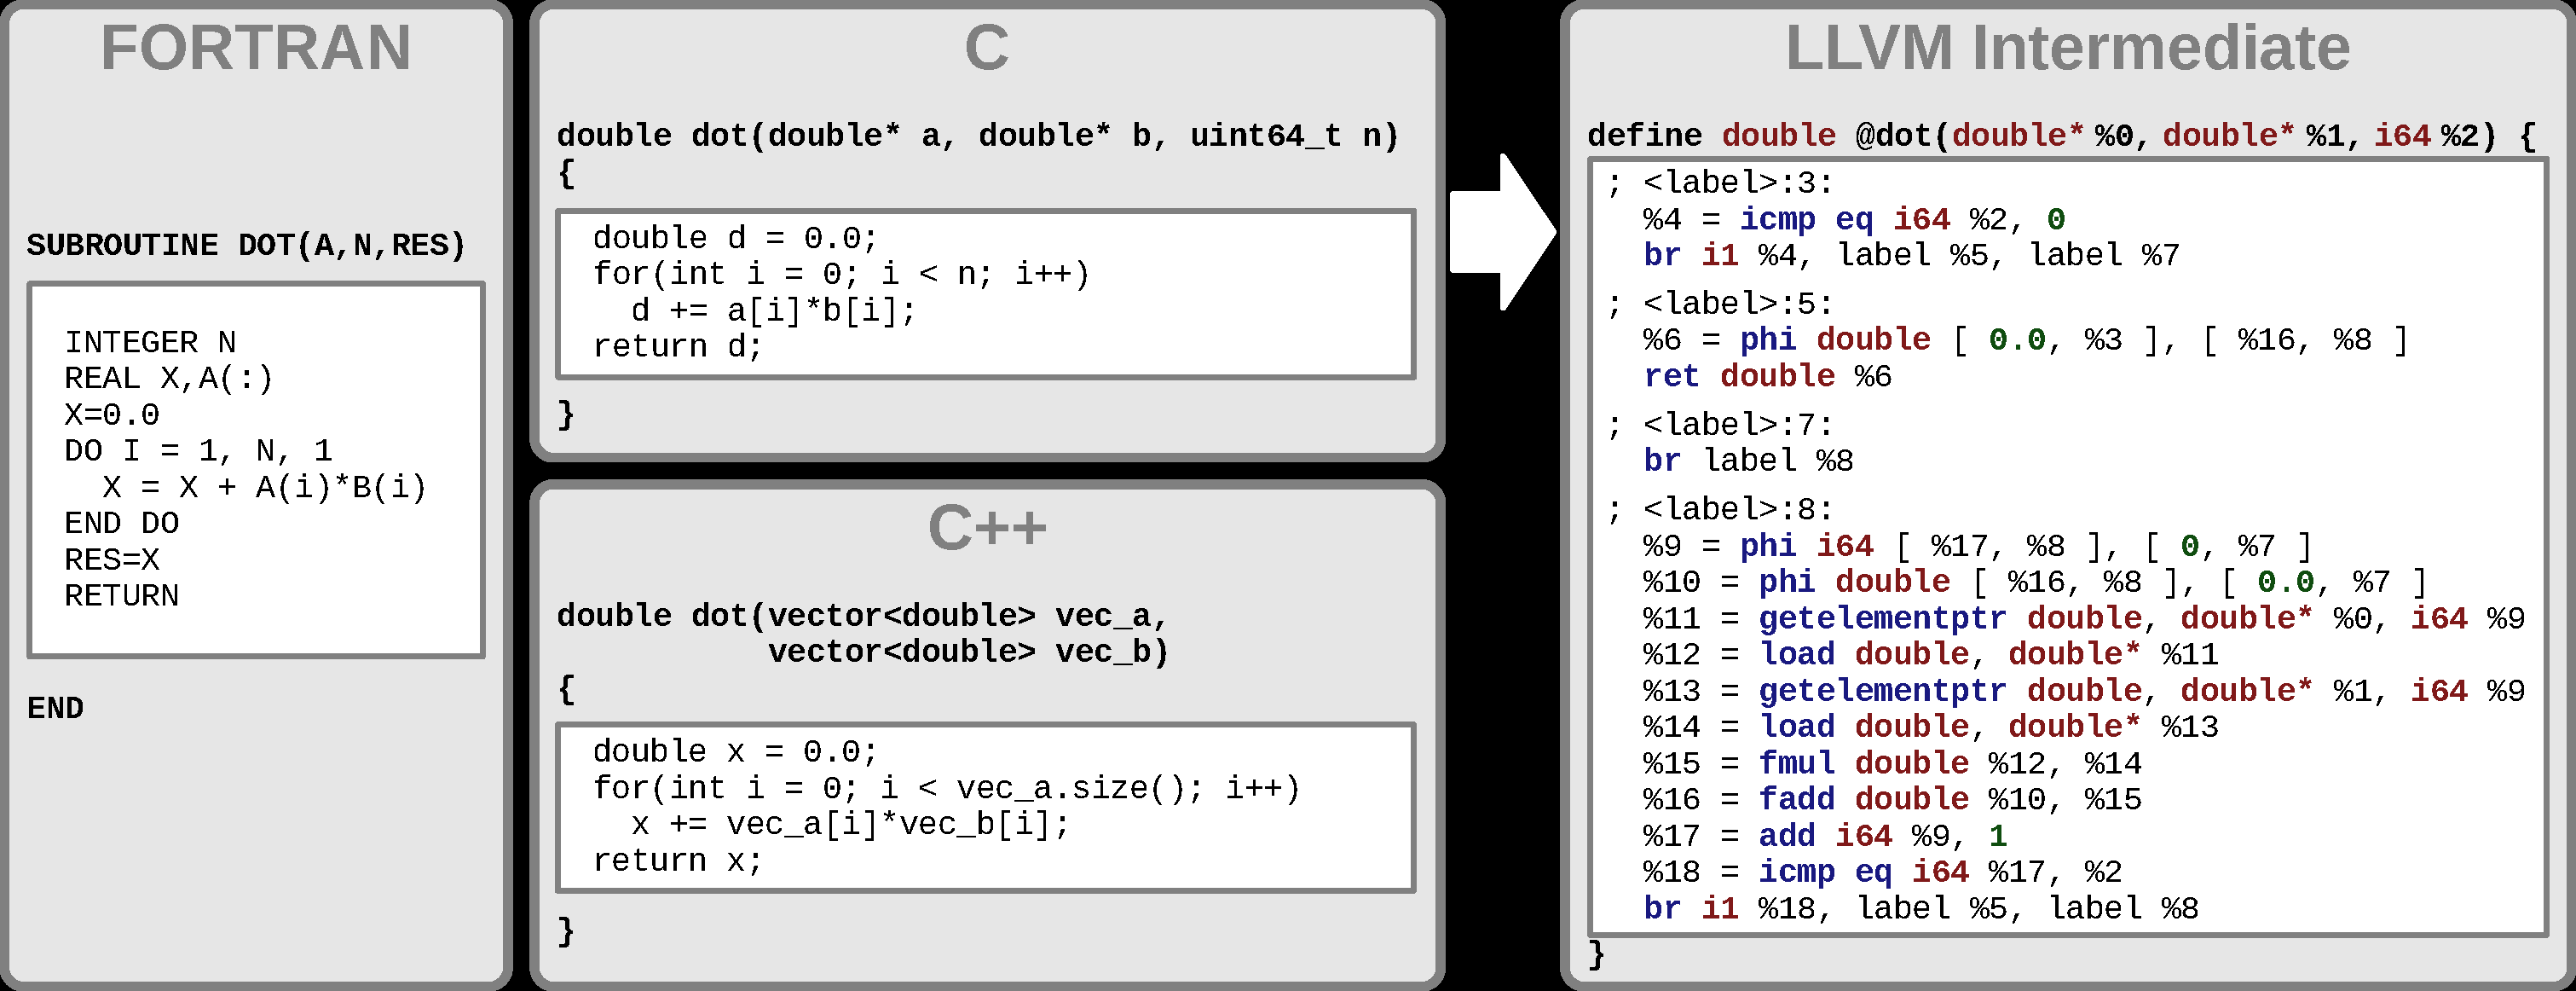
\includegraphics[width=\columnwidth]{figures/model_representations_textual}
\end{blackbox}

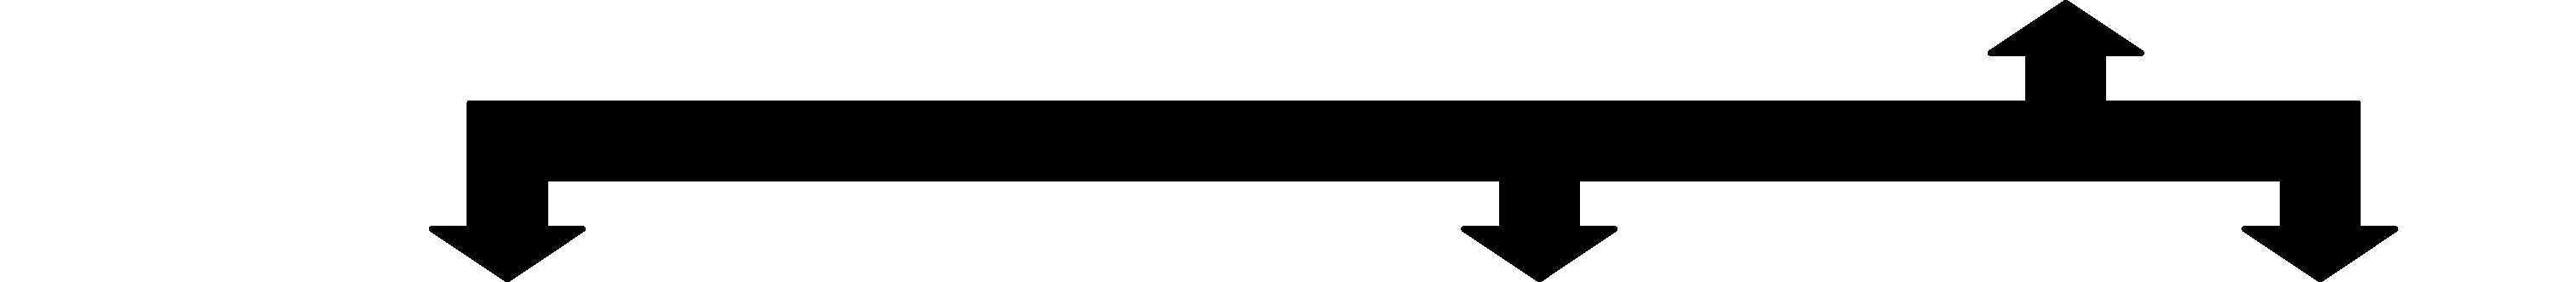
\includegraphics[width=\columnwidth]{figures/model_arrows_upper}

\begin{blackbox}{Data Structure Representation}
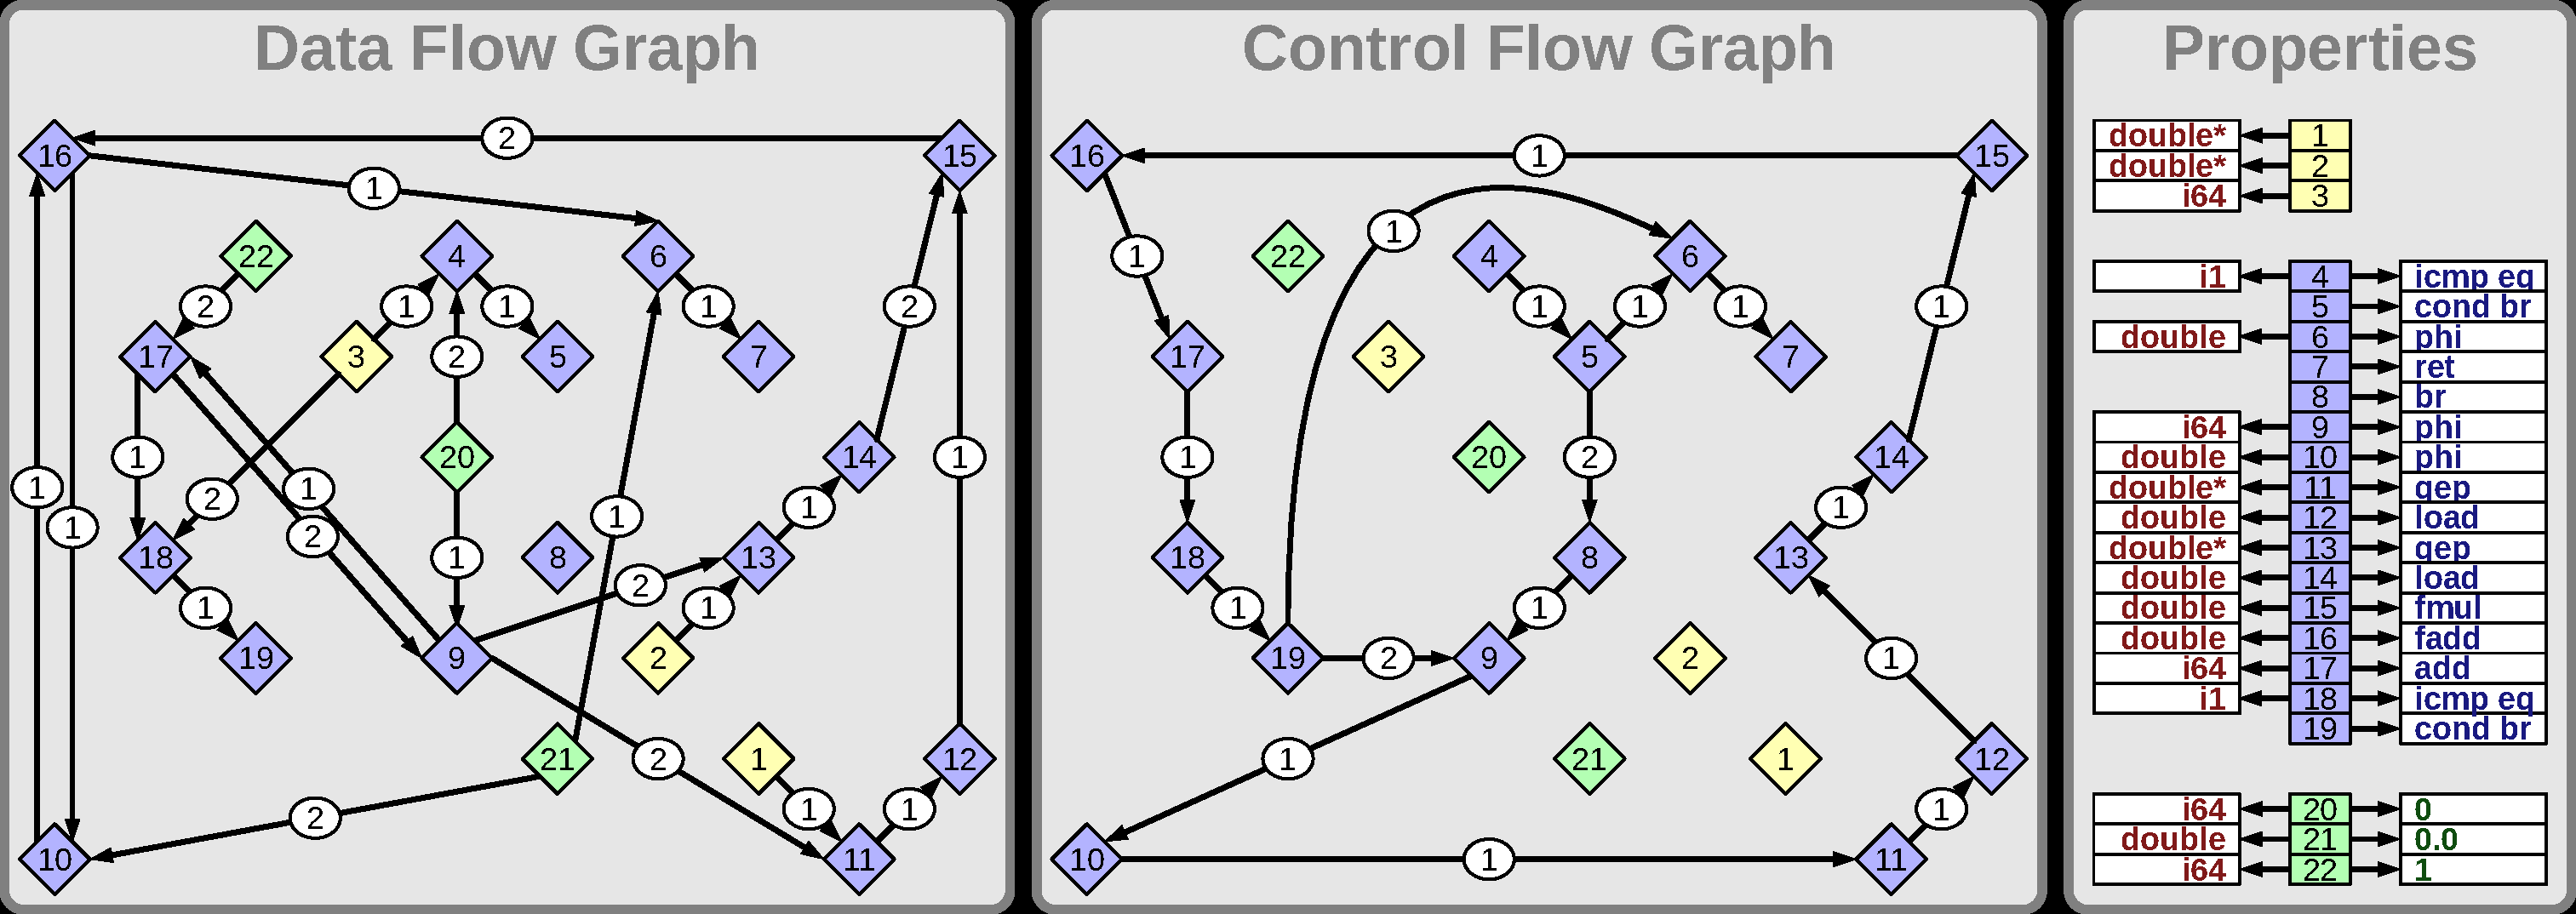
\includegraphics[width=\columnwidth]{figures/model_representations_structure}
\end{blackbox}

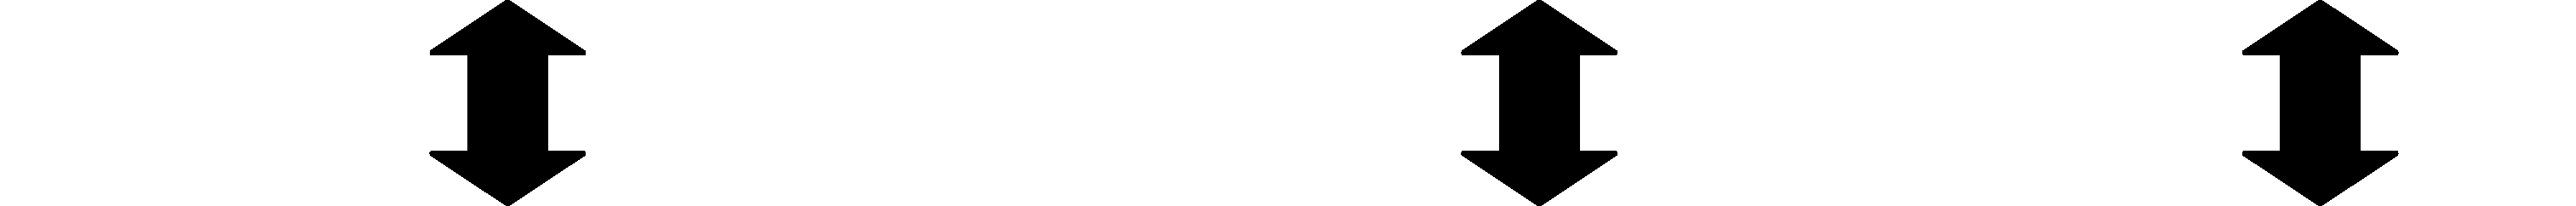
\includegraphics[width=\columnwidth]{figures/model_arrows_lower}

\begin{blackbox}{Mathematical Representation}
    \centering
    \begin{minipage}{0.329\textwidth}
        \begin{graybox}
            \scriptsize
            \setlength{\abovedisplayskip}{0pt}
            \setlength{\belowdisplayskip}{0pt}
            \vspace{-0.5em}
            \begin{align*}
                DF&G_\mathcal F=\{(1,11,1),(2,13,1)\\[-0.5em]
                  &(3,4,1),(3,18,2),(4,5,1),\\[-0.5em]
                  &(6,7,1),(9,11,2),(9,13,2),\\[-0.5em]
                  &(9,17,1),(10,16,1),(11,12,1),\\[-0.5em]
                  &(12,15,1),(13,14,1),(14,15,2),\\[-0.5em]
                  &(15,16,2),(16,6,1),(16,10,1),\\[-0.5em]
                  &(17,9,2),(17,18,1),(18,19,1),\\[-0.5em]
                  &(20,4,2),(20,9,1),(21,6,1),\\[-0.5em]
                  &(21,10,2),(22,17,2)\}\subset\mathbb N^3
            \end{align*}
        \end{graybox}
    \end{minipage}
    \begin{minipage}{0.329\textwidth}
        \begin{graybox}
            \scriptsize
            \setlength{\abovedisplayskip}{0pt}
            \setlength{\belowdisplayskip}{0pt}
            \vspace{-0.5em}
            \begin{align*}
                CFG_\mathcal F=\{&(4,5,1),(5,6,1),\\[-0.5em]
                  &(5,8,2),(6,7,1),\\[-0.5em]
                  &(8,9,1),(9,10,1),\\[-0.5em]
                  &(10,11,1),(11,12,1),\\[-0.5em]
                  &(12,13,1),(13,14,1),\\[-0.5em]
                  &(14,15,1),(15,16,1),\\[-0.5em]
                  &(16,17,1),(17,18,1),\\[-0.5em]
                  &(18,19,1),(19,6,1),\\[-0.5em]
                  &(19,9,2)\}\subset\mathbb N^3
            \end{align*}
        \end{graybox}
    \end{minipage}
    \begin{minipage}{0.329\textwidth}
        \centering
        \begin{graybox}
            \scriptsize
            \setlength{\abovedisplayskip}{0pt}
            \setlength{\belowdisplayskip}{0pt}
            \vspace{-0.5em}
            \begin{align*}
                T_\mathcal F={}&\{(1,\textit{double*}),(2,\textit{double*}),\dots\}\\[-0.5em]
                      \subset{}&\mathbb N\times Types_\text{LLVM}\\[-0.25em]
                P_\mathcal F={}&\{1,2,3\}\subset\mathbb N\\[-0.25em]
                I_\mathcal F={}&\{(4,\textit{icmp eq}),(5,\textit{cond br}),\dots\}\\[-0.5em]
                      \subset{}&\mathbb N\times Opcodes_\text{LLVM}\\[-0.25em]
                G_\mathcal F={}&\{\}\subset\mathbb N\\[-0.25em]
                C_\mathcal F={}&\{(20,0),(21,0),(22,1)\}\\[-0.5em]
                      \subset{}&\mathbb N\times\mathbb R
            \end{align*}

            \vspace{0.45em}
        \end{graybox}
    \end{minipage}

    \begin{minipage}{0.55\textwidth}
        \begin{graybox}
            \setlength{\abovedisplayskip}{0pt}
            \setlength{\belowdisplayskip}{0pt}
            \vspace{-0.5em}
            \begin{align*}
                M_{dot}=(DFG_\mathcal{F},
                 CFG_\mathcal{F},
                 T_\mathcal{F},
                 P_\mathcal{F},
                 I_\mathcal{F},
                 G_\mathcal{F},
                 C_\mathcal{F})
            \end{align*}
        \end{graybox}
    \end{minipage}
\end{blackbox}
\caption{Compiler-generated LLVM IR code is decomposed into data flow, control
         flow and per-value attributes.
         Mathematical notations of the three components are shown at the
         bottom.}
\label{fig:derivemaths}
\end{figure}

\section{Constraint Programming on SSA Programs}

    With a mathematical model of SSA programs in place, properties of such
    programs can now be formulated as constraint problems.
    For this purpose, \autoref{not:modelrepresentations} is introduced first,
    followed by the actual definition of {\em SSA constraint problem}s in
    \autoref{def:cprob}.

\begin{notation}{Set of SSA Models}{modelrepresentations}
    Given a specific SSA representation (LLVM, Hydrogen, MIR, $\dots$), then
    denote $F$ the set of all valid functions that can be expressed in it.

    The {\em set of SSA models} $\mathcal M$ is defined as
    \begin{align*}
        \mathcal M := \{M\mid\exists\mathcal F\in F\colon M
                        \text{ is the SSA Model of }\mathcal F\}
    \end{align*}
\end{notation}

\begin{definition}{SSA constraint problem}{cprob}
    An SSA constraint problem $C=(V,P)$ is made up of a finite set of variables
    $V$ and a boolean predicate
    $P\colon\mathbb N^V\times\mathcal M\mapsto\{\text{true}, \text{false}\}$.
    The set of {\em constraint solutions} for a given constraint problem and a
    specific SSA model $M\in\mathcal M$ is given as
    \begin{align*}
        S(C,M) = \{s\in\mathbb N^V\mid P(s,M)=\text{true}\}.
    \end{align*}
\end{definition}

    Some intuition is required here.
    The predicate function $P$ takes two arguments, firstly a tuple of integers
    and secondly a model of a function.
    The finite set $V$ identifies the elements withing the tuples, it can be
    thought of as a set of labels.
    The tuples of integers in $\mathbb N^V$ correspond to tuples of values
    within the function.
    The predicate function determines whether these values stand in a specific
    relationship to each other.
    Finally, the set of constraint solutions lists all those tuples, for which
    the predicate holds.

    The two parameters of $P$ -- integer tuple and model -- should be
    interpreted as two very different beasts here.
    The predicate evaluates whether a condition holds for the tuple of integers,
    the model on the other hand serves as the context for this evaluation.
    This is reflected in the definition of the set of constraint solutions,
    which is the set of all {\em true} evaluations given a fixed model.
    More pointedly, it makes sense to query ``all loops in a given function'',
    yet to ask for ``all functions with a specific loop'' is meaningless.

    The interesting aspect of this defition is now the structure of predicates
    $P$.
    This section will concern it self with how meaningful predicates can be
    composed from small building blocks and how the internal structure of the
    predicate can lead to efficient solver approaches.
    In order to evoke an intuition about these challenges, there will first be
    an example.

\subsection{Constraint Program Example}

\begin{figure}[t]
\centering
{\huge $S\left(C,M\right)=$}
\vspace{0.5em}

$\text{\huge S}\left(\left(
\begin{minipage}{0.3\textwidth}
\setlength{\abovedisplayskip}{0pt}
\begin{align*}
    V=\{\text{phi}, \text{update}, \text{step}\},
\end{align*}
\begin{align*}
    P&(x,\mathcal F)=\left((x_\text{step},1)\in C_\mathcal{F}\right.\\
    &\land(x_\text{phi},x_\text{update})\in DFG_\mathcal{F}^*\\
    &\land(x_\text{step},x_\text{update})\in DFG_\mathcal{F}^*\\
    &\land(x_\text{phi}, phi)\in I_\mathcal{F}\\
    &\land(x_\text{step}, add)\in I_\mathcal{F}\\
    &\left.\land(x_\text{update},x_\text{phi})\in DFG_\mathcal{F}^*\right)
\end{align*}
\end{minipage}
\right)\text{\huge ,}\left(
\begin{minipage}{0.5\textwidth}
\setlength{\abovedisplayskip}{0pt}
\begin{align*}
DF&G_\mathcal F=\{(1,2,1),(4,5,1),(6,8,2),\\
&(6,10,2),(6,14,1),(7,13,1),(8,9,1),\\
&(9,12,1),(10,11,1),(11,12,2),\dots\},\\
CF&G_\mathcal F=\{(1,2,1),(2,4,1),(2,3,2),\\
&(3,6,1),(4,5,1),(6,7,1),(7,8,1),\\
&(8,9,1),(9,10,1),(10,11,1),\dots\},\\
I_\mathcal F&{}=\{(1,icomp\ eq),(2,cond\ br),\dots\}\\
T_\mathcal F&{}=\{(1,i1),(4,double),(6,i64),\dots\}\\
C_\mathcal F&{}=\{(17,0),(18,0),(19,1)\}\\
P_\mathcal F&{}=\{20,21,22\}\\
G_\mathcal F&{}=\{\}
\end{align*}
\end{minipage}
\right)\right)$

\vspace{0.5em}
{\huge$=\{\{\text{phi}:6,\text{update}:14,\text{step}:19\}\}\subset\mathbb N^V$}

\caption{Simple loop iterators are identified in the model from
         \autoref{fig:derivemaths}.
         On the left is the formulation of loop iterators as a predicate
         composed of six statements over three variables.
         Applied to the model on the right, one solution corresponding to
         the source variable {\tt i} is found.}
\label{fig:constraintsolution}
\end{figure}

    Consider the task of detecting in a program all simple loop counters.
    Such loop counters show up in LLVM IR as data flow cycles of a phi node
    and an add instruction.
    This is expressed as an SSA constraint problem on the left side of
    \autoref{fig:constraintsolution}, with the variables
    $V=\{\text{phi}, \text{update}, \text{step}\}$ and a predicate $P$ that
    describes the conditions that the variables have to adhere to.

    This decomposes the predicate into logical conjunctions of a range of
    {\em elemt-of} relationships that operate on the structures of the model.
    With this decomposition, an algorithmic solution to the constraint problem
    is accessible, and the set of solutions for a given SSA program can be
    determined.
    This SSA constraint problem is applied to the {\tt dot} function in
    \autoref{fig:derivemaths}, as visible on the right side of the figure.

    The set of constraint solutions contains a single element, the tuple
    $\{\text{phi}:6,\text{update}:14,\text{step}:19\}$.
    This solution can be mapped back onto the LLVM IR code shown at the top of
    \autoref{fig:derivemaths}, from which the model was derived.
    The value {\tt phi} maps to the $\Phi$ node $\%9$, the value {\tt update}
    maps to $\%14$ and the value {\tt step} maps to the constan $1$.
    These are of course the instructions generated from the loop structure of
    the original program.
    Furthermore, this is indeed the only loop to be detected.

\subsection{Solving of SSA Constraint Problems}

    The aim of a solver for SSA constraint problems is to compute the set of
    solutions $S(C,M)$ for some concrete values of $C$ and $M$.
    This is fundamentally a search problem: the space of $\mathbb N^V$ has to be
    searched for values satisfying $P$.
    The size of $\mathbb N^V$, wich is countable but infinite, requires
    non-trivial computational approaches to this problem, even when the direct
    evaluation of $P$ can be efficiently performed.

    On top of that, an algorithmic solution requires an intelligent way to
    encode the boolean predicate.
    It is intuitive and well established in literature to use backtracking for
    solving constraint problems, so firstly this will be reformulated
    recursively as follows.
    The finite set of $V$ can be enumerated $V=\{v_0,v_1,\dots,v_n\}$.

    Then consider $C_k=(V_k,P_k)$, where $P_k$ is defined as
    \begin{align*}
        P_k(x)=\left\{\begin{array}{l}\text{true} if P(x,y)=true for some y\\
                                      \text{false} otherwise\end{array}\right.
    \end{align*}

    Consider the following purely algebraic reformulation.
    \begin{align*}
        S_k=\{\emptyset\}\\
        S_{k+1}(C,\mathcal F)=&\{s\in\mathbb N^V_k\mid P(s,\mathcal F)=\text{true}\}\\
                             =&\{
    \end{align*}

\subsection{Structure of SSA Constraint Problems}

    Predicates for useful SSA constraint problems are composed by logical
    connectors from a limited set of {\em atomic} predicates, that cannot
    further be decomposed.
    The atomic predicates are defined directly on the mathematical model and
    they often only utilize a very small set of variables, typically one or two.
    Many of then are simple element-of relationships for the different
    components in the SSA model.
    In the previous example, this was true for all the atomic constraints.

    There are some important compiler analysis problems that can not not be
    decomposed with logical connectors into atomic predicates using only one
    or two variables.
    They are mostly concerned with graph properties and we will discuss some of
    them in detail later in this chapter.
    For the purposes of constraint solving, these are more difficult to handle.

    Via the logical connectors $\land$ and $\lor$, the atomic predicates
    interact on their shared variables.
    There will be some additional high level connectors introduced later, which
    appriximate logical operators from first order logic.

\section{Implementation of Constraint Predicates}

    With the solver approach derived, it now needs to be established how real
    constarint problem predicates can be algorithmically implemented in order
    to evaluate the required functions.

\subsection{Important Graph Properties}

    With our established notation, we can now transfer standard compiler
    analysis problems into this more formal language.
    Most of these are based on graph theoretic considerations, so we
    will firstly need to recapitulate some graph theory basics.
    Firstly, there is the notion of {\em cuts} of graphs, that we will introduce
    here in a hybrid version of edge based and vertex based modelling.

    \begin{definition}{Connections and Cuts}{def:cuts}
        Consider an adjacency set $E\subset\mathbb{N}\times\mathbb{N}$ of a
        directed graph and let $a,b\in\mathbb{N}$.
        \newline
        A {\em connection} between $a$ and $b$ in $E$ is a subset
        $A\subset\mathbb{N}$ such that a finite sequence $c_1,\dots,c_n$
        exists with
        \begin{gather*}
            a=c_1\hspace{1cm}c_2,\dots,c_{n-1}\in A\hspace{1cm}b=c_n\\
            (c_k,c_{k+1})\in E\hspace{1em}\text{for all}\hspace{1em}k=1,\dots,n-1.
        \end{gather*}
        A {\em cut} between $a$ and $b$ in $E$ is a subset $B\subset E$
        such that no {\em connection} between $a$ and $b$ in $E\setminus B$
        exists.
        We define the {\em set of cuts} between $a$ and $b$ in $E$ as
        \begin{align*}
            \text{Cuts}_E(a,b):=\{B\subset E\mid B\text{ is {\em cut} between $a$ and $b$ in $E$}\}
        \end{align*}
    \end{definition}

    These notions are quite intuitive, two vertices in a graph have a connection
    if one can reach the other via the available edges and by ``cutting'' these
    edges, they are no longer connected.

    These definitions are very useful in order to identify crucial properties of
    data and control flow graphs.
    Most standard is the the definition of a dominator in the control flow
    graph: An instruction $d$ is said to dominate another instruction $n$ if
    every path from the entry node to $n$ through the control flow graph must
    go through $d$.
    In our model this is of course equivalent to the following:

    \begin{definition}{Dominator}{def:dominator}
        Consider an instruction $n$ in a function $\mathcal F$.
        A {\em dominator} of $n$ in $\mathcal{F}$ is an instruction $d$ such
        that $\{(d,m)\mid(d,m)\in CFG_\mathcal{F}^*\}$ is a {\em cut} between $1$ and $n$ in $CFG_\mathcal{F}^*$.
    \end{definition}

    Another important definition is the concept of control dependence.
    Control dependence models the behaviour of conditional control flow.
    Instructions that are executed only in some control flow paths are control
    dependent on the conditional branches that preceed them.

    \begin{definition}{Control Dependence}{cdg}
        Consider instructions $a,b$.
        We say that an $b$ is control dependent on $a$ if a instructions
        $c,c'$ exist such that $(a,c),(a,c')\in CFG_\mathcal{F}^*$ and
        \begin{align*}
            \{(a,c)\}\in{}&{}\text{Cuts}_E(a,b)\\
            \{(a,c')\}\notin{}&{}\text{Cuts}_E(a,b)\text{.}
        \end{align*}
        We define the {\em control dependence graph} as follows
        \begin{align*}
            CDG_\mathcal{F}:=\{(a,b)\in\mathbb{N}^2\mid b\text{ control dependent on }a\}
        \end{align*}
    \end{definition}

\begin{figure}[p]
    \centering
    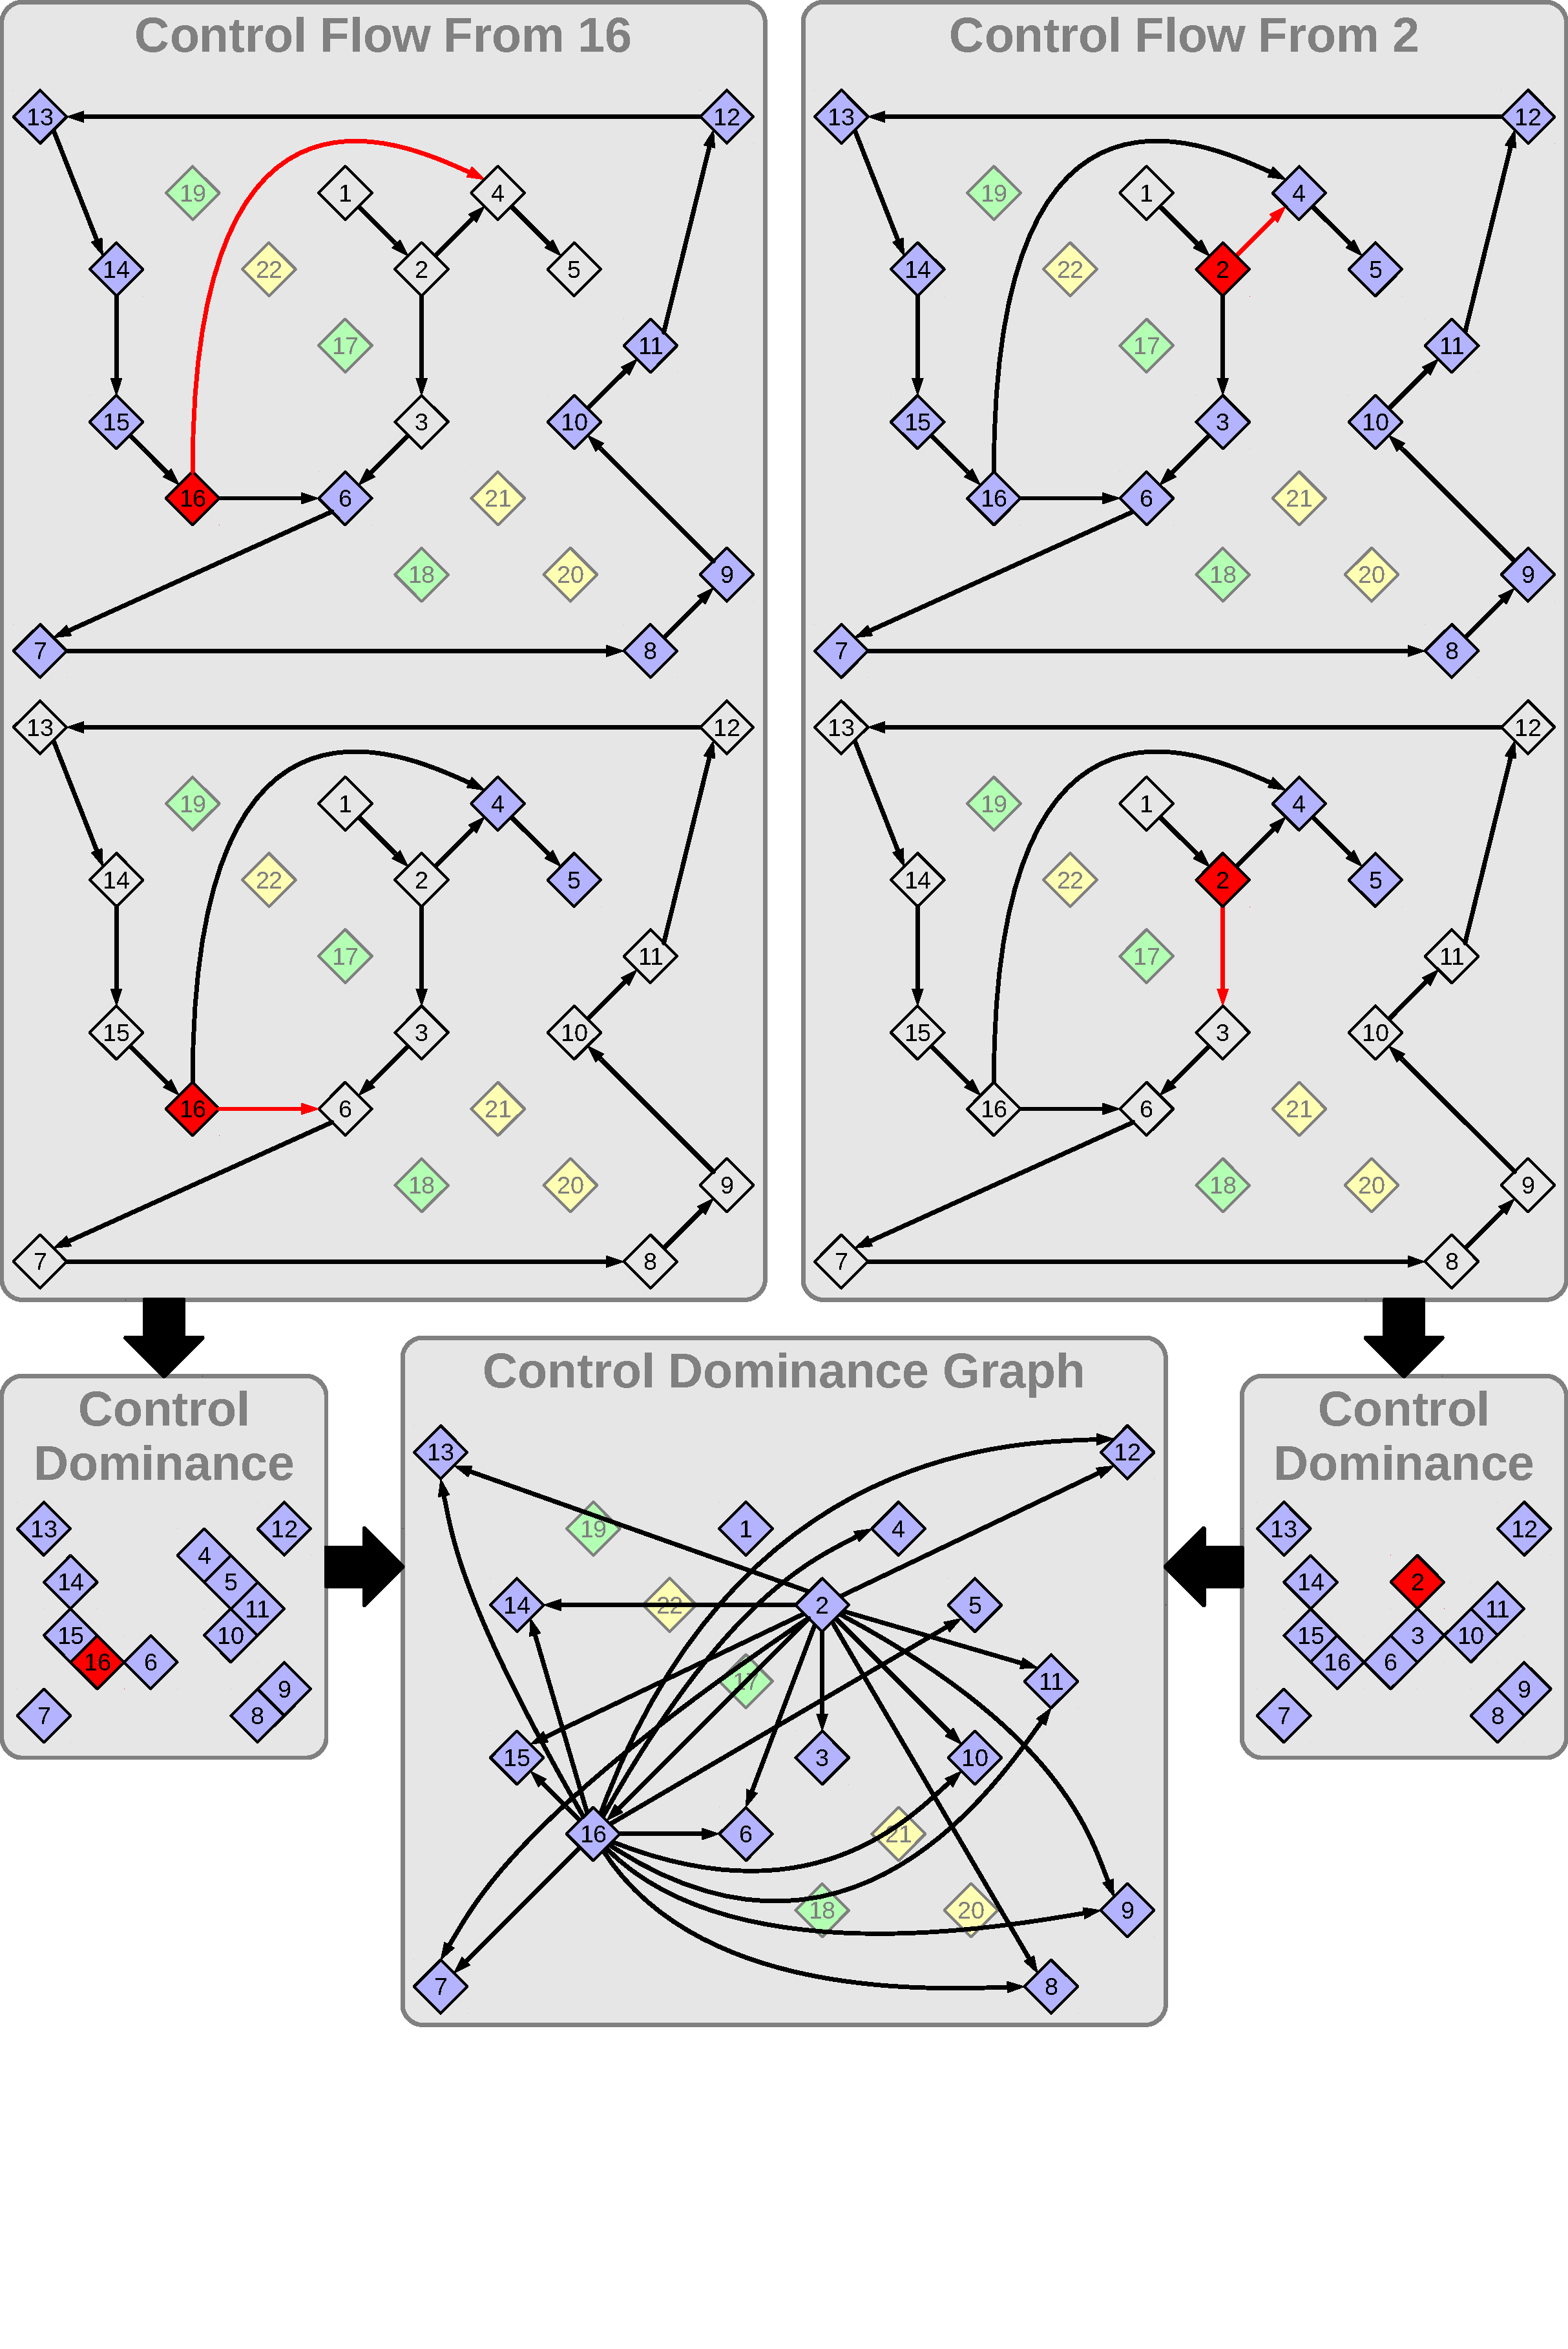
\includegraphics[width=\textwidth,height=1.5\textwidth]{figures/schaubild2.pdf}

    \vspace{27.38136pt}
    \caption{Computation of the control dependence graph.}
    \label{fig:pdg}
\end{figure}

\subsection{Control Dependence Example}

    The control dependence graph is a function of the control flow graph, as is
    directly apparent from \autoref{def:cdg}.
    We can see how an example control dependence graph is computed in
    \autoref{fig:pdg}, from the control flow graph of the \texttt{dot} function
    in \autoref{fig:derivemaths}.
    From the definition it is immediately obvious that we need to only consider
    conditional branches as origins of control dependence.

    We can consider the two conditional branches $2$ and $16$ independently.
    On the right, we consider only $2$.
    We check the defining property: On the top of the figure, all the
    instructions that are not reachable from $2$ without the edge $(2,4)$ are in
    grey.
    Below this, all instructions not reachable from $2$ without $(2,3)$ are
    grey.
    We see that $4,5$ are always reachable and $1$ is never reachable, these are
    therefore not control dependent on $2$.
    All the other instructions are control dependent on $2$.

    Once we have computed this for all conditional branches, we take the union
    on graphs and get the complete control dependence graph of the function.
    Note what this graph represents:
    Once the loop in the function has been unrolled, it contains a conditional
    and a loop.
    Eveything within the body of the conditional is control dependent on $2$.
    Everythig within the loop as well as everything afterwards is control
    dependent on $16$.

\subsection{Phi Dependence Graph}

    Phi nodes are fundamental in single static assignment form and need special
    care.
    The value that a phi node takes depends on from where a phi node was
    reached.
    We need to encapsulate this in a graph.

    \begin{definition}{Phi Dependence Graph}{def:pog}
        Let $p$ a phi node and $c$ a conditional branch instruction.
        We say that the outcome of $p$ depends on $c$ if there is a branch
        instruction $b$ that reaches $p$ such that $b$ is control dependent on
        $c$.

        This defines the {\em phi dependence graph} $\Phi DG_\mathcal{F}$.
    \end{definition}

\subsection{Program Dependence Graph}

    After the control flow, data flow and control dependence graph, we lastly
    introduce the {\em program dependence graph}.
    It is the most exhaustive tool that we have to describe how values depend on
    each other.

    \begin{definition}{Program Dependence Graph}{def:pdg}
        The {\em program dependence graph} is defined as the union of data flow
        and control dependence graphs.
        \begin{align*}
            PDG_\mathcal{F}:=DFG_\mathcal{F}^*\cup CDG_\mathcal{F}^*\cup\Phi DG_\mathcal{F}\text{.}
        \end{align*}
    \end{definition}

    With the program dependence graph, we can now define subsections of the
    program that are self-contained and can be separated into their own
    function.
    This works even if they contain complicated control flow.
    Firstly, we need a definition of an interface.

    \begin{definition}{Interface}{def:interface}
        Let $a\in CFG_\mathcal{F}^*$ and $b_1,\dots,b_n\in DFG_\mathcal{F}^*$.
        Furthermore let $A\subset\mathbb{N}$ a set of instructions.

        We say that $(b_1,\dots,b_n)$ is an interface to $A$ if it is a cut
        between $o$ and $A$ in $PDG_\mathcal{F}$ for any of the following $o$:
        \begin{itemize}
            \item $o$ is a paramter
            \item $o$ is impure
        \end{itemize}
    \end{definition}

\newpage
\subsection{Interface Example}

    We will now consider a non-trivial example.
    Consider this snppet of C code, implementing a function that performs a
    simple square root approximation on each element in an array of double
    precision floating point values.

\begin{figure}[ht]
\begin{lstlisting}[language=C]
void map_sqrt(size_t length, double* array)
{
    for(int i = 0; i < length; i++)
    {
        double root = 1.0;
        for(int i = 0; i < 10; i++)
            root = 0.5*(root+array[i]/root);

        array[i] = root;
    }
}
\end{lstlisting}
\caption{{\bf map$\circ$sqrt}: Apply an appriximate sqare root function to each
         element in a vector.}
\end{figure}

    Coneptually, we should be able to disentangle the square root function from
    the control flow of the outer loop.
    This is possible with the preceeding definition of {\em interfaces}.

\newpage
In single static assignment form, this code looks as follows:

\begin{lstlisting}[language=LLVM]
define void @map_sqrt(i64, double*) {
  %3 = icmp eq i64 %0, 0
  br i1 %3, label %5, label %4

; <label>:4:
  br label %6

; <label>:5:
  ret void

; <label>:6:
  %7 = phi i64 [ %10, %8 ], [ 0, %4 ]
  br label %12

; <label>:8:
  %9 = getelementptr double, double* %1, i64 %7
  store double %19, double* %9
  %10 = add nuw i64 %7, 1
  %11 = icmp eq i64 %10, %0
  br i1 %11, label %5, label %6

; <label>:12:
  %13 = phi i64 [ 0, %6 ], [ %20, %12 ]
  %14 = phi double [ 1.0, %6 ], [ %19, %12 ]
  %15 = getelementptr inbounds double, double* %1, i64 %13
  %16 = load double, double* %15
  %17 = fdiv double %16, %14
  %18 = fadd double %14, %17
  %19 = fmul double %18, 5.0
  %20 = add nuw nsw i64 %13, 1
  %21 = icmp eq i64 %20, 10
  br i1 %21, label %8, label %12
}
\end{lstlisting}

    In this example, the set $\{\%9\}$ is an interface to $\{(\%19,\%store)\}$.

\section{Formulating Constraint Problems}

    With this mathematical background, it is now possible to derive constraint
    programming on top of LLVM code.

    Consider the following definitions of simple binary predicates:

    \begin{align*}
     is\_branch\_inst(\mathcal F, n):= (n,\text{\bf br})\in T_\mathcal{F}\\
     is\_control\_edge(\mathcal F, n, m):= (n,m)\in CFG_\mathcal{F}^*\\
     is\_control\_dom(\mathcal F, n, m):= \\
    \end{align*}

    We can then use these predicates to define more complex constructs, such as
    single entry, single exit (SESE) regions.

    \begin{definition}{}{}{}
        A single entry single exit region is a tuple $a,b,c,d\in\mathcal N$ such
        that the following properties hold:
        \begin{align*}
            is\_control\_edge(\mathcal{F},a,b)\\
            is\_control\_edge(\mathcal{F},c,d)\\
            is\_control\_dom(\mathcal{F},c,d)\\
            is\_control\_postdom(\mathcal{F},d,c)\\
        \end{align*}
    \end{definition}
